
\documentclass[aspectratio=169]{beamer}

% Use your collegeBeamer theme when it is available. Otherwise, compile with a clean fallback theme.
\IfFileExists{collegeBeamer.sty}{%
    \usepackage[polyu,en]{collegeBeamer}
}{%
    \usetheme{Madrid}
    \usecolortheme{default}
    \setbeamertemplate{navigation symbols}{}
    \setbeamertemplate{footline}[frame number]
    \newcommand{\QApage}{%
        \begin{frame}[plain]
            \centering
            \vfill
            {\Huge Questions?}\\[0.8em]
            {\large Thank you for listening.}
            \vfill
        \end{frame}}
}

\usepackage[T1]{fontenc}
\usepackage[utf8]{inputenc}
\usepackage{lmodern}
\usepackage{graphicx}
\usepackage{booktabs}
\usepackage{tabularx}
\usepackage{array}
\usepackage{amsmath}
\usepackage{xcolor}
\usepackage{tikz}
\usetikzlibrary{arrows.meta,positioning,shapes.geometric,calc,fit}

\graphicspath{{assets/}{./assets/}}

\definecolor{phriBlue}{HTML}{0055A4}
\definecolor{phriCyan}{HTML}{2E9CCA}
\definecolor{phriOrange}{HTML}{F28C28}
\definecolor{phriGreen}{HTML}{3D9970}
\definecolor{phriGray}{HTML}{555555}
\definecolor{lightBlue}{HTML}{EAF4FB}
\definecolor{lightOrange}{HTML}{FFF1E5}
\definecolor{lightGreen}{HTML}{EAF6F0}
\definecolor{lightGray}{HTML}{F3F4F6}

\newcommand{\keypoint}[1]{\textbf{\textcolor{phriBlue}{#1}}}
\newcommand{\smallcite}[1]{\textcolor{phriGray}{\scriptsize #1}}
\newcommand{\tightlist}{\setlength{\itemsep}{0.32em}\setlength{\parskip}{0pt}}
\newcommand{\miniheader}[1]{\vspace{0.2em}\textbf{\textcolor{phriBlue}{#1}}}

% Include  figures when the assets folder is available.
% If the figure file is missing, the slide still compiles and shows the expected path.
\newcommand{\paperfig}[3][]{%
    \IfFileExists{#2}{%
        \includegraphics[#1]{#2}%
    }{%
        \fbox{%
        \begin{minipage}[c][0.44\textheight][c]{0.88\linewidth}
            \centering
            \textcolor{phriGray}{\Large Missing original figure}\\[0.4em]
            \texttt{\detokenize{#2}}\\[0.4em]
            \scriptsize Put the paper's \texttt{assets/} folder next to this \texttt{.tex} file.
        \end{minipage}}%
    }%
    \par\vspace{0.25em}{\scriptsize\textcolor{phriGray}{#3}}%
}

\title{Physical Human--Robot Interaction: \\A Review from the Guide Robot Perspective}
\subtitle{ICHMS 2026 }
\author{Yufa You \and Hailong Huang}
\institute{Department of Aeronautical and Aviation Engineering\\The Hong Kong Polytechnic University}
\date{Department of Aeronautical and Aviation Engineering\\The Hong Kong Polytechnic University}

\begin{document}

% 0:00--0:25
\maketitle

\section{Motivation}

% 0:25--1:15
\begin{frame}{Motivation}
\vspace{-0.5em}
\begin{columns}[T,onlytextwidth]
    \begin{column}{0.42\textwidth}
        \scriptsize
        \textbf{\textcolor{phriBlue}{Why HRI / pHRI now?}}
        \begin{itemize}
            \setlength{\itemsep}{0.12em}
            \setlength{\parskip}{0pt}
            \item Human-only work is becoming not efficient enough.
            \item Full autonomy has not yet been achieved in many complex tasks.
            \item HRI is a stage that we have to face.
        \end{itemize}


        \vspace{0.15em}
        \textbf{\textcolor{phriBlue}{Why guide robots?}}\\
        \begin{itemize}
            \setlength{\itemsep}{0.12em}
            \setlength{\parskip}{0pt}
            \item Guide-robot demands can be mapped to general pHRI.
            \item Guide-robot research has broad application value.
        \end{itemize}
        
    \end{column}

    \begin{column}{0.55\textwidth}
        \centering
        \paperfig[height=0.74\textheight]{assets/1.pdf}{Fig.~1: guide-robot demands mapped to general pHRI and application domains.}

        \vspace{0.15em}
        \begin{beamercolorbox}[wd=0.92\linewidth, sep=3pt]{block body example}
        \scriptsize
        \textbf{Review contribution:}\quad
        three-stage review, cross-stage diagnosis, and two future directions.
        \end{beamercolorbox}
    \end{column}
\end{columns}
\end{frame}

\section{Three-stage Review}

% 1:15--1:55
\begin{frame}{Representative works to three stages}
\vspace{-0.5em}
\centering
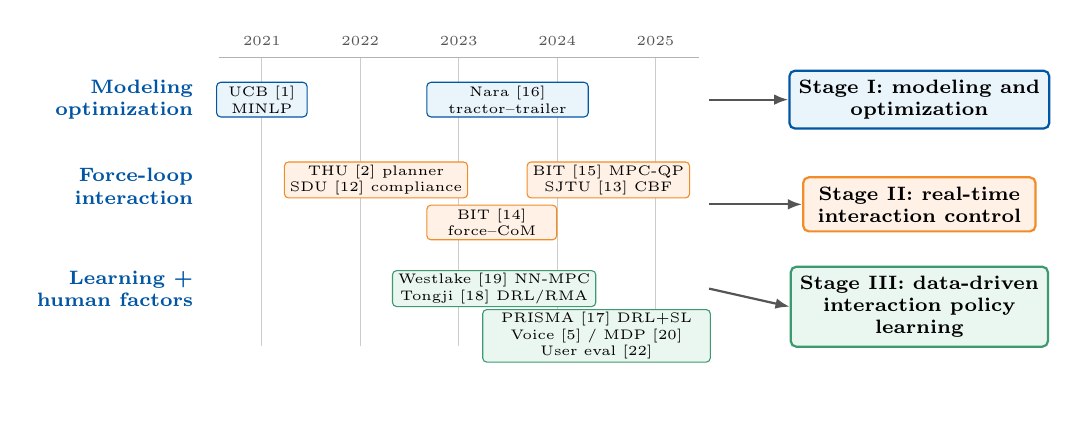
\begin{tikzpicture}[
    font=\scriptsize,
    year/.style={font=\tiny, text=phriGray},
    lane/.style={font=\scriptsize\bfseries, text=phriBlue, anchor=east, align=right},
    work/.style={rounded corners=1.5pt, minimum height=0.44cm, inner xsep=2pt, inner ysep=1pt, align=center, font=\tiny},
    stage/.style={rounded corners=2pt, thick, minimum width=2.95cm, minimum height=0.68cm, align=center, font=\scriptsize\bfseries},
    arr/.style={-{Latex[length=1.8mm]}, thick, phriGray}
]
% Year axis.
\foreach \x/\year in {2.1/2021,3.35/2022,4.6/2023,5.85/2024,7.1/2025}{
    \node[year] at (\x,0.12) {\year};
    \draw[phriGray!30] (\x,-0.08) -- (\x,-3.75);
}
\draw[phriGray!45] (1.55,-0.08) -- (7.65,-0.08);

% Three condensed evidence lanes.
\node[lane] at (1.35,-0.62) {Modeling\\optimization};
\node[work, draw=phriBlue, fill=lightBlue, minimum width=1.15cm] at (2.1,-0.62) {UCB [1]\\MINLP};
\node[work, draw=phriBlue, fill=lightBlue, minimum width=2.05cm] at (5.22,-0.62) {Nara [16]\\tractor--trailer};

\node[lane] at (1.35,-1.72) {Force-loop\\interaction};
\node[work, draw=phriOrange, fill=lightOrange, minimum width=1.7cm] at (3.55,-1.64) {THU [2] planner\\SDU [12] compliance};
\node[work, draw=phriOrange, fill=lightOrange, minimum width=1.65cm] at (5.02,-2.18) {BIT [14]\\force--CoM};
\node[work, draw=phriOrange, fill=lightOrange, minimum width=1.9cm] at (6.50,-1.64) {BIT [15] MPC-QP\\SJTU [13] CBF};

\node[lane] at (1.35,-3.02) {Learning +\\human factors};
\node[work, draw=phriGreen, fill=lightGreen, minimum width=1.85cm] at (5.05,-3.02) {Westlake [19] NN-MPC\\Tongji [18] DRL/RMA};
\node[work, draw=phriGreen, fill=lightGreen, text width=2.75cm] at (6.35,-3.62) {PRISMA [17] DRL+SL\\Voice [5] / MDP [20]\\User eval [22]};

% Review abstraction.
\node[stage, draw=phriBlue, fill=lightBlue] (s1) at (10.45,-0.62) {Stage I: modeling and\\optimization};
\node[stage, draw=phriOrange, fill=lightOrange] (s2) at (10.45,-1.95) {Stage II: real-time\\interaction control};
\node[stage, draw=phriGreen, fill=lightGreen] (s3) at (10.45,-3.25) {Stage III: data-driven\\interaction policy\\learning};
\draw[arr] (7.78,-0.62) -- (s1.west);
\draw[arr] (7.78,-1.95) -- (s2.west);
\draw[arr] (7.78,-3.02) -- (s3.west);

\node[align=center, text width=11.8cm, font=\scriptsize] at (6.15,-4.35) {
    % \textbf{Review logic:} the three-stage view is a mechanism-based abstraction of these works.
};
\end{tikzpicture}
\end{frame}

% 1:15--2:05
\begin{frame}{Comparations}
\begin{columns}[T,onlytextwidth]
    \begin{column}{0.5\textwidth}
        \centering
        \paperfig[width=0.98\linewidth]{assets/2_1.pdf}{ Fig.~2(a): technical evolution timeline.}
    \end{column}
    \begin{column}{0.5\textwidth}
        \centering
        \paperfig[width=0.98\linewidth]{assets/2_2.pdf}{ Fig.~2(b): cross-comparison of key characteristics.}
    \end{column}
\end{columns}
\vspace{0.3em}
\begin{block}{Details}
Core ideas, strengths and limitations.
\end{block}
\end{frame}

% 2:05--2:50
\begin{frame}{Stage I: modeling and optimization}
\begin{columns}[T,onlytextwidth]
    \begin{column}{0.50\textwidth}
        \scriptsize
        \begin{block}{Core idea}
        Describe the problem using a cost function, constraints, and differential equations, and then solve it as an optimization problem.
        \end{block}
        \begin{block}{Strength}
        Strong interpretability and long-horizon prediction.
        \end{block}
        \miniheader{Representative mechanisms}
        \begin{itemize}\tightlist
            \item Taut--slack leash switching models.
            \item Human--robot force--motion relationships.
            \item MPC and search-based planning.
        \end{itemize}
        \smallcite{Refs: Xiao [1], Chen [2], Hong [9].}
    \end{column}

    \begin{column}{0.46\textwidth}
        \scriptsize
        
        \vspace{-0.15em}
        \begin{block}{Limitation}
        Sensitive to model bias; finite-horizon optimization can get stuck in local optima.
        \end{block}
        \vspace{-0.15em}
        \miniheader{MPC local-trap example}
        \vspace{0.05em}
        \begin{columns}[T,totalwidth=\linewidth]
            \begin{column}{0.49\linewidth}
                \centering
                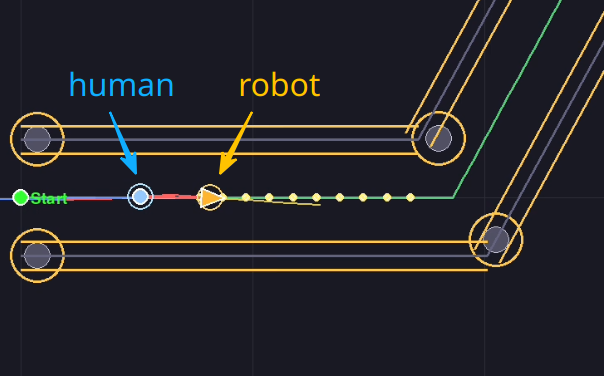
\includegraphics[width=\linewidth,height=0.3\textheight,keepaspectratio]{assets/mpc1.png}\\[-0.15em]
                {\tiny feasible path}
            \end{column}
            \begin{column}{0.49\linewidth}
                \centering
                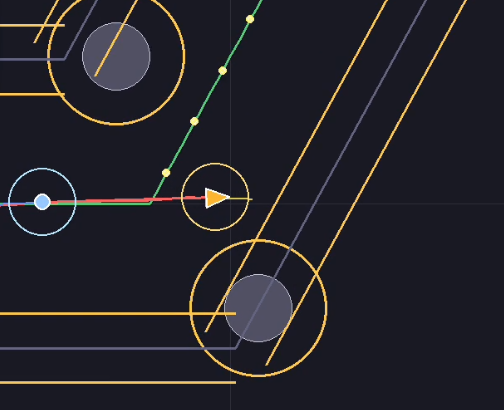
\includegraphics[width=\linewidth,height=0.3\textheight,keepaspectratio]{assets/mpc2.png}\\[-0.15em]
                {\tiny local trap}
            \end{column}
        \end{columns}
        \vspace{0.05em}
        \smallcite{Failure: local minimum; little forward progress.}
        \begin{beamercolorbox}[wd=0.92\linewidth, sep=3pt]{block body example}
        \scriptsize
        \textbf{Optimal but not ideal}\quad
        \end{beamercolorbox}
        
    \end{column}
\end{columns}
\end{frame}

% 2:50--3:35
\begin{frame}{Stage II: real-time interaction control}
\begin{columns}[T,onlytextwidth]
    \begin{column}{0.50\textwidth}
        \begin{block}{Core idea}
        Use force sensors or force estimators, and then design force planning or compliance control.
        \end{block}
        \centering
        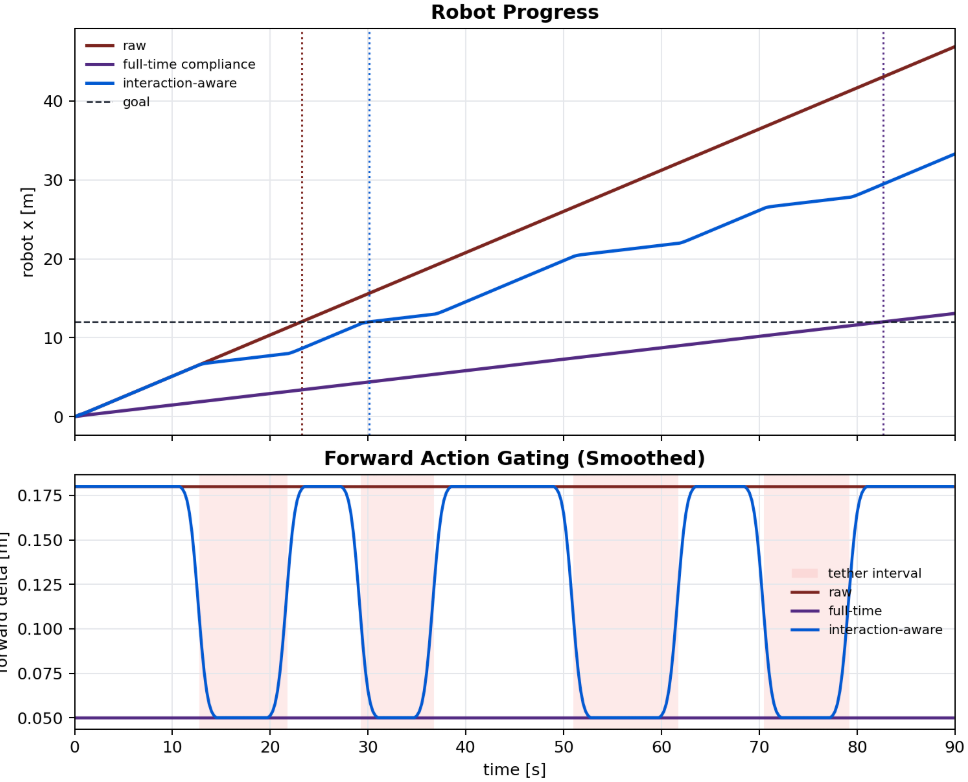
\includegraphics[width=0.82\linewidth]{assets/compliance.png}\\[-0.15em]
    \end{column}
    \begin{column}{0.46\textwidth}
        \begin{block}{Strength}
        Natural, stable, and responsive physical interaction.
        \end{block}
        \begin{block}{Limitation}
        Not globally optimal and maybe time-consuming.
        \end{block}
        \scriptsize
        \miniheader{Typical components}
        \begin{itemize}\tightlist
            \item Impedance / admittance control.
            \item Force observers and online parameter identification.
            \item MPC and control barrier functions for local safety.
        \end{itemize}

        \vspace{0.1em}
        \raggedright
        \smallcite{Representative works: Du et al. [12]; Fan et al. [13]; Gu et al. [14,15]; Akhdan et al. [16].}
    \end{column}
\end{columns}
\end{frame}

% 3:35--4:20
\begin{frame}{Stage III: data-driven policy learning}
\begin{columns}[T,onlytextwidth]
    \begin{column}{0.50\textwidth}
        \begin{block}{Core idea}
        Learn complex dynamics and distributions from data or simulation.
        \end{block}
        \miniheader{Main technical routes}
        \begin{itemize}\tightlist
            \item Reinforcement learning for policy optimization.
            \item TCN / LSTM models for behavior prediction.
            \item Hybrid adaptation: RMA, teacher--student learning, NN-MPC.
        \end{itemize}
    \end{column}
    \begin{column}{0.46\textwidth}
        \begin{block}{Strength}
        Captures nonlinear behavior and individual differences.
        \end{block}
        \begin{block}{Limitation}
        Data demand, interpretability, safety verification, and sim-to-real gap.
        \end{block}
        \smallcite{Representative works: Aliotta et al. [17]; Ma et al. [18]; Zhou et al. [19]; Kim et al. [20].}
    \end{column}
\end{columns}
\end{frame}

\section{Diagnosis and Future Directions}

% 4:20--5:05
\begin{frame}{Cross-stage diagnosis: what is still missing?}
\scriptsize
\begin{tabularx}{\textwidth}{>{\raggedright\arraybackslash}p{2.2cm}XXX}
\toprule
 & \textbf{Stage I} & \textbf{Stage II} & \textbf{Stage III} \\
\midrule
Main strength & Interpretable long-horizon planning & Real-time compliance and comfort & Adaptive nonlinear behavior learning \\
Main weakness & Model bias and heavy optimization & Weak global foresight & Data demand and weak verification \\
Typical output & Single optimized trajectory & Local compliant response & Learned policy or predictor \\
Risk in guidance & Uncomfortable or delayed response & Myopic behavior & Unsafe or unexplainable action \\
\bottomrule
\end{tabularx}
\vspace{0.6em}
\begin{columns}[T,onlytextwidth]
    \begin{column}{0.48\textwidth}
        \begin{block}{Bottleneck 1}
        \textbf{Long-term efficiency vs. real-time interaction} are not jointly optimized across time scales.
        \end{block}
    \end{column}
    \begin{column}{0.48\textwidth}
        \begin{block}{Bottleneck 2}
        Most methods produce \textbf{single-solution behavior}, but we do need a plan B for something unpredictable.
        \end{block}
    \end{column}
\end{columns}
\end{frame}

% 5:05--6:05
\begin{frame}{Future direction I: hybrid architecture of learning and optimization}
\begin{columns}[T,onlytextwidth]
    \begin{column}{0.42\textwidth}
        \begin{block}{Why hybrid?}
        \begin{itemize}\tightlist
            \item Learning handles \keypoint{uncertain human states}: intention, preference, parameters.
            \item Optimization/control handles \keypoint{constraints}: safety, stability, feasibility.
            \item The key is clear division of module responsibility.
        \end{itemize}
        \end{block}
        \begin{block}{Design principle}
        Learning proposes or identifies; model-based control verifies and executes.
        \end{block}
    \end{column}
    \begin{column}{0.55\textwidth}
        \centering
        \paperfig[width=0.98\linewidth]{assets/3.pdf}{ Fig.~3: learning--optimization fusion architectures.}
    \end{column}
\end{columns}
\end{frame}

% 6:05--7:20
\begin{frame}{Future direction II: multimodal planning and global optimality}
\begin{columns}[T,onlytextwidth]
    \begin{column}{0.42\textwidth}
        \begin{block}{Why multimodal?}
        Under the same goal, a user may go left, go right, slow down, or temporarily resist guidance.
        \end{block}
        \scriptsize

        \miniheader{Desired capability}
        \begin{itemize}\tightlist
            \item Generate multiple feasible candidates.
            \item Evaluate comfort, safety, and task progress.
            \item Select consistently in real time.
        \end{itemize}
        \begin{block}{Open problem}
        Policy diversity must be paired with safety boundaries and closed-loop stability.
        \end{block}
    \end{column}
    \begin{column}{0.50\textwidth}
        \centering
        \paperfig[width=0.98\linewidth]{assets/4.pdf}{ Fig.~4: mainstream routes for multimodal planning.}
    \end{column}
\end{columns}
\end{frame}

% 7:20--8:00
\begin{frame}{Conclusion}
\begin{block}{1. Review contribution}
This review contributes a \keypoint{three-stage review}, a \keypoint{cross-stage diagnosis}, and \keypoint{two future directions}.
\end{block}

\begin{block}{2. From guide robots to pHRI}
Insights from guide robots generalize to pHRI and a broader range of application scenarios.
\end{block}
\end{frame}

\QApage

\end{document}
